
%(BEGIN_QUESTION)
% Copyright 2010, Tony R. Kuphaldt, released under the Creative Commons Attribution License (v 1.0)
% This means you may do almost anything with this work of mine, so long as you give me proper credit

Suppose a voltmeter connected between test points {\bf D} and {\bf F} registers 5 V in this circuit:

$$\includegraphics[width=15.5cm]{i03294x01.eps}$$

Identify the likelihood of each specified fault for this circuit.  Consider each fault one at a time (i.e. no coincidental faults), determining whether or not each fault could independently account for {\it all} measurements and symptoms in this circuit.

% No blank lines allowed between lines of an \halign structure!
% I use comments (%) instead, so that TeX doesn't choke.

$$\vbox{\offinterlineskip
\halign{\strut
\vrule \quad\hfil # \ \hfil & 
\vrule \quad\hfil # \ \hfil & 
\vrule \quad\hfil # \ \hfil \vrule \cr
\noalign{\hrule}
%
% First row
{\bf Fault} & {\bf Possible} & {\bf Impossible} \cr
%
\noalign{\hrule}
%
% Another row
$R_1$ failed open &  &  \cr
%
\noalign{\hrule}
%
% Another row
$R_2$ failed open &  &  \cr
%
\noalign{\hrule}
%
% Another row
$R_3$ failed open &  &  \cr
%
\noalign{\hrule}
%
% Another row
$Q_1$ failed open &  &  \cr
%
\noalign{\hrule}
%
% Another row
$R_1$ failed shorted &  &  \cr
%
\noalign{\hrule}
%
% Another row
$R_2$ failed shorted &  &  \cr
%
\noalign{\hrule}
%
% Another row
$R_3$ failed shorted &  &  \cr
%
\noalign{\hrule}
%
% Another row
$Q_1$ failed shorted &  &  \cr
%
\noalign{\hrule}
%
% Another row
Voltage source dead &  &  \cr
%
\noalign{\hrule}
} % End of \halign 
}$$ % End of \vbox


\vfil 

\underbar{file i03294}
\eject
%(END_QUESTION)





%(BEGIN_ANSWER)

This is a graded question -- no answers or hints given!

%(END_ANSWER)





%(BEGIN_NOTES)

This circuit tends to frighten many students, because they don't see how to quantitatively approach it.  The current mirror's job is to regulate current at a value of 5 mA, but it's hard to calculate how much total current will be in the circuit with the 1 k$\Omega$ resistor $R_1$ in parallel with the current mirror.  How much current will go through $R_1$, since we have no known voltage drop to apply in Ohm's Law?  How can we figure out $R_1$'s voltage drop if we don't know how much voltage $R_2$ and $R_3$ drop (since we don't know the total current)?

We could apply a network theorem such as Superposition, but that's nothing more than a higher-power quantitative approach.  What we should really do is apply a more general problem-solving technique.

\vskip 10pt

One such problem-solving technique is to {\it simplify the problem}: identify whatever it is that's causing you confusion and remove that thing from the problem to make the problem simpler.  Then, after we have analyzed the simpler problem, we might arrive at some insight helpful for solving the original problem.  One thing we could choose to remove from this particular problem is the entire current mirror network, leaving only three resistors and a voltage source.  If we were to do this, it should become immediately apparent that all three resistors will carry 6 milliamps of current, dropping 6 volts each.  Now, whatever the current mirror does in this circuit, it should be apparent that it will provide another path for current in parallel with $R_1$.  This means that in a healthy circuit, we should expect to see {\it more} than 6 milliamps of current through $R_2$ and $R_3$.

The exact amount of current we should expect to see through $R_2$ and $R_3$ is not terribly relevant, because it's significantly more than what we apparently have going through $R_3$ with only 5 volts drop measured across it.  In fact, a measurement of 5 volts between points D and F suggests a current of only 5 mA through the 1 k$\Omega$ resistance of $R_3$.  We know that there should be more current than this, and therefore more voltage drop between points D and F as well, because the current mirror's regulated current of 5 mA should add with whatever amount of current goes through $R_1$.  Since we have less current going through $R_3$ than we would expect under normal operating conditions, the most likely fault is an {\it open} fault in the circuit somewhere.

If the current mirror were failed open, the amount of current through $R_3$ would be 6 mA as previously determined.  This is more than we measured, and so the likely culprit is a failed-open $R_1$, which would result in only the current mirror's 5 mA going through $R_3$ and causing the 5 volt drop between points D and F.

% No blank lines allowed between lines of an \halign structure!
% I use comments (%) instead, so that TeX doesn't choke.

$$\vbox{\offinterlineskip
\halign{\strut
\vrule \quad\hfil # \ \hfil & 
\vrule \quad\hfil # \ \hfil & 
\vrule \quad\hfil # \ \hfil \vrule \cr
\noalign{\hrule}
%
% First row
{\bf Fault} & {\bf Possible} & {\bf Impossible} \cr
%
\noalign{\hrule}
%
% Another row
$R_1$ failed open & $\surd$ &  \cr
%
\noalign{\hrule}
%
% Another row
$R_2$ failed open &  & $\surd$ \cr
%
\noalign{\hrule}
%
% Another row
$R_3$ failed open &  & $\surd$ \cr
%
\noalign{\hrule}
%
% Another row
$Q_1$ failed open &  & $\surd$ \cr
%
\noalign{\hrule}
%
% Another row
$R_1$ failed shorted &  & $\surd$ \cr
%
\noalign{\hrule}
%
% Another row
$R_2$ failed shorted &  & $\surd$ \cr
%
\noalign{\hrule}
%
% Another row
$R_3$ failed shorted &  & $\surd$ \cr
%
\noalign{\hrule}
%
% Another row
$Q_1$ failed shorted &  & $\surd$ \cr
%
\noalign{\hrule}
%
% Another row
Voltage source dead &  & $\surd$ \cr
%
\noalign{\hrule}
} % End of \halign 
}$$ % End of \vbox



%INDEX% Troubleshooting review: electric circuits

%(END_NOTES)


